\documentclass[a4paper,11pt,twocolumn]{article}
\usepackage{lingmacros}
\usepackage{blindtext}
\usepackage{tree-dvips}
\usepackage{amsmath}
\usepackage{multicol}
\usepackage{mathtools}
\usepackage{hyperref}
\usepackage{graphicx}
\usepackage{amssymb}
\usepackage[table]{xcolor}
\graphicspath{ {./Latex/} }

%\pagestyle{headings} Writes the heading on top of the page.
\begin{document}

\title{Logistic regression and neural networks}
\date{2019\\ October}
\author{Eirik Nordgård\\ Geophysical Institute,\ University of Oslo}


\twocolumn[
\begin{@twocolumnfalse}
\maketitle
\begin{abstract}
Here you can write your abstract

\end{abstract}

All material for this project may be found on 
\url{https://github.com/eirikngard/FYS-STK4155/tree/master/Project_2}

\end{@twocolumnfalse}
]
\

\section{Introduction}

In this project credit card data with 23 features is used to determine whether the clients will default or not default their debt. The data output thus is binary, 1 for default and 0 for not default, and prediction these includes solving a classification problem. In this project this is done using logistic regression and neural networks. Overall, the main goal is to assess which model best predicts the outcome based on the 23 features in the data, and how adjusting parameters of these models affect the result. The performance is measured by the accuracy score, which simply is a measure of how often the given model predict correct outcome. Accuracy score ranges from 0 to 1, 1 being a perfect classifier.    
\begin{gather*}
Accuracy = \frac{\sum\limits_{i=1}^n I(y_i = y_i)}{n}
\end{gather*}
\\

\section{Theory}


\subsection{Logistic regression}

Logistic regression is used to solve classification problems. These are problems concerning outcomes, $y_i$, in form of discrete variables. Commonly the classification problems in question has two possible outcomes, true or false. Using the credit card data as an example, the two outcomes would be if a client would pay his/hers debt or not. This type of outcome is often calleed binary outcome, and can easily be programmed as 1 or 0.

The dependent variables (outcomes) $y_i$ are discrete, ranging from $k=0,...,K-1$ where $K$ is classes. The main goal is to predict the output classes from a designmatrix $\hat{X} \in \mathbb{R}^{nXp}$ made of \textit{n} samples carrying \textit{p} features/predictors. The simplest output is perhaps a binary output, only having values 0 or 1 meaning yes/no, true/false, pay/dont pay etc. From there it is desired to identify the classes to which new unseen samples belong. 

A descrete output can be obtained in several ways, but the simplest may be to have a sign function, which maps the output of a linear regressor to values ${0,1}, f(a)=sign(a) = 1$ if $a$ $\geq$ 0 and 0 if otherwise.  Although this model is very simple, in many cases it might be convenient to know the probability of an output belonging a given caegory rather than a single value. This is done using the \textit{logistic function}, and is often called a "soft classifier".  The classifier outputs the probability of $x_i$ belonging to a category $y_i=\{0,1\}$. In this case the classifier is given by a \textit{Sigmoid} function, often reffered to as a likelihood function. The Sigmoid function $p(y)$ is given by\cite{slides}

\begin{equation}
p(y) = \frac{1}{1+e^{-y}}  = \frac{e^y}{1+e^y}
\label{p1}
\end{equation}

and looks like this 

\begin{figure}[h]
\centering
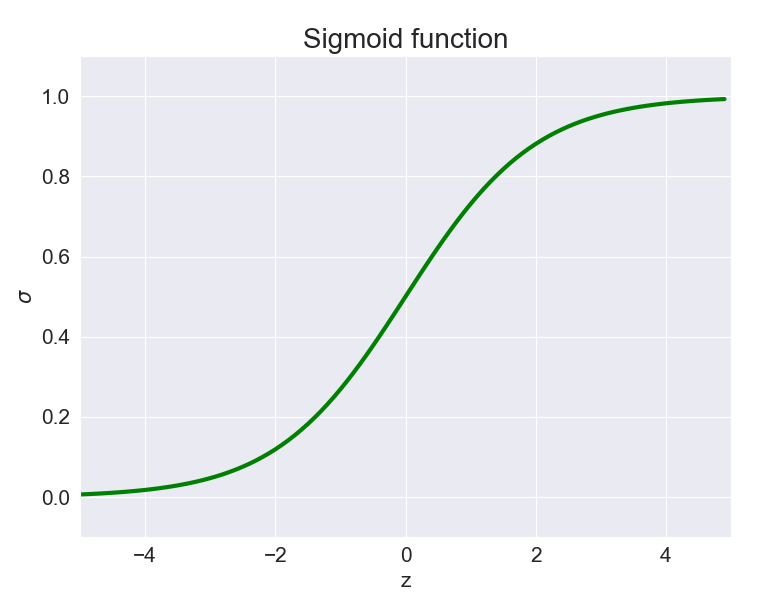
\includegraphics[scale=0.75]{Sigmoid}
\caption{Plain Sigmoid as example of likelihood function}
\label{Sigmoid}
\end{figure}

Like other likelihoods,  eq. \eqref{p1} here we have that the likelihood  $p(y_i = 0) = 1-p(y_i = 1) $, always resulting in a summed likelihood of 1. Assuming two classes $y_i$  being either 0 or 1, we have

\begin{equation}
\label{y1}
y_i=\beta_0+\beta_1x_i+...+\beta_nx_i
\end{equation}

Used in in eq.\eqref{p1}, this gives 

\begin{equation}
\label{y2}
p(y_i=1\mid x_i,\hat{\beta}) = \frac{e{\beta_0+\beta_1x_i}}{1+e{\beta_0+\beta_1x_i}}
\end{equation}
and 
\begin{equation}
\label{y3}
p(y_i=0\mid x_i,\hat{\beta}) = 1 - p(y_i=1\mid x_i\hat{\beta})
\end{equation}

Eq. \eqref{y2} and eq. \eqref{y3} can then be used to find the maximum likelihood of an event. The product of all individual probabilities of a specific outcome $y_i$ is used to obtain a log-likelihood function, which in turn gives the cost function 

\begin{equation}
\begin{multlined}
C(\hat{\beta})=\sum\limits_{i=1}^{n}\big(y_i\: log\: p(y_i=1\vert x_i,\hat{\beta})\\ 
+(1-y_i)\:log\: \big[1-p(y_i=1\vert x_i,\hat{\beta}\big]\big)
\end{multlined}
\label{c1}
\end{equation}

Eq. \eqref{c1} is called the \textit{cross entropy}. Being convex, a local minimizer of this function will also be a global minimizer. Hence, minimizing eq. \eqref{c1} with respect to each $\beta$ gives 


\begin{equation}
\frac{\partial\hat{\beta}}{\partial\beta_0}=
-\sum\limits_{i=1}^n\big(y_i-\frac{e^{\beta_0+\beta_1x_i}}{1+e^{\beta_0+\beta_1x_i}}\big)
\label{min1}
\end{equation}
and 
\begin{equation}
\frac{\partial\hat{\beta}}{\partial\beta_1}=
-\sum\limits_{i=1}^n\big(y_ix_i-x_i\frac{e^{\beta_0+\beta_1x_i}}{1+e^{\beta_0+\beta_1x_i}}\big)
\label{min2}
\end{equation}

It is worth mentioning that far from all cost functions are convex. Many cost functions used in machine learning are in fact non-convex and of high dimensionality. Compressing eq. \eqref{min1} and eq. \eqref{min2} we get the following expressions for the first derivative. This is the gradient used in the gradient descent method explained later.

\begin{equation}
\frac{\partial C(\hat{\beta})}{\partial\hat{\beta}}=-\hat{X}^T(\hat{y}-\hat{p})
\label{compcost1}
\end{equation}

%\begin{equation}
%\frac{\partial^2C(\hat{\beta})}{\partial\hat{\beta}\partial%\hat{\beta}^T}=\hat{X}^T\hat{W}\hat{X}
%\label{compcost2}
%\end{equation}

where $\hat{y}$ is a vector with n elements $y_i$, the $n x p$ matrix $\hat{X}$ containing the $x_i$ values and the vector $\hat{p}$ is the fitted probabilities $p(y_i\mid x_i,\hat{\beta})$.
%and 
%$\hat{W}$ being a diagonal matrix with elements $p(y_i\mid xi,%\hat{\beta})(1-p(y_i\mid xi,\hat{\beta})$. These derivatives %are used to create the Hessian matrix, later used to solve the %minimization problem. Unlike in linear regression, solving %these for $\hat{\beta}$ now requires a gradient descent method
\footnote{here is a paragraph on Hessian. check if i use this later}
\cite{slides}. 

\subsection{Gradient Descent Method}

The idea of a gradient descent (GD) method is that a function $F(x)$, with $x=x_1,...,x_n$, decreases fastest if one goes from $x$ in the direction of the negative gradient $-\nabla F(x)$. If 
\begin{equation}
x_{v+1}=x_v-\gamma_v\nabla F(x_v)
\label{GD1}
\end{equation}
where $\gamma_v$ is called learning rate or step length, in this case $\gamma_v>0$. The gradient used in eq. \eqref{GD1} is obtained by eq. \eqref{compcost1}. For small enough $\gamma_v$ we will then have $F(x_{v+1}\geq F(x_v)$, meaning we are always moving towards smaller values and eventually a minimum of F \cite{slides}.
\\ 
Choosing appropriate learning rate is important. If chosen too small the method will converge very slowly, and chosen too large may result in unpredictable behaviour. The first step doing the GD is to make a guess $x_0$ for a minimum of F. Note that the minima is a global minima only if the function is a convex function. 

\textbf{Logistic regresseion er som et neuralt nettverk uten layers.} 
\footnote{Make sure p (sigmoid) is defined somewhere above}
\cite{slides}. 

\subsubsection{Standard/Steepest Gradient Descent}
I have used this as the first gradient descent. Iterate 1000, calculated the gradient, minimizing the cost function. This iteration outputs betas, used to make prediction of y. Thereafter y is used in the sigmoid function to classify the data og default or not. Making a threshold of 0,5, where sigmoid output of less than 0,5 is 0, and above is 1. Then I count how many of the predicted values match with the values of the data y (last column in data set) to get the accuracy score for this gradient descent.  

\subsubsection{Stochastic Gradient Descent}

Write about epocs and minibatches. Why we use them, how we use them and maby how to optimize the number of these? 

Anyhow, I have used stochastic gradient descent with linear regression as well, and found it to be around 1% more accurate on the training data than the stnadard gradient descent. 

\subsection{Artificial Neural Networks}

Artificial Neural Networks (ANN) is a computational system that by training on examples can learn to perform tasks. Increasing the number of examples the ANN can learn from will increase the accuracy of the tasks performed. It is called artificial neural network because it is supposed to mimic a biological system such as a brain, where neurons interact by sending signals in the form of mathematical functions. The ANN is constructed in layers containing an arbitrary number of neutrons, which in turn is connected by a weight variable. Similarly to an actual brain, the neurons in a ANN can only communicate with each other if the incoming signal exceeds a certain threshold value. If the signal is "strong" enough, an output is sent forward, but if this activation threshold is not reached the neuron remain inactive, providing zero output\cite{slides}. 
\\

The neurons described above may be on different forms. One type of artificial neuron is called the \textit{perceptron}, and it has the general form 

\begin{equation}
y = \sigma (\sum\limits_{i=1}^n w_ix_i + b_i) = \sigma (z)
\label{neu1}
\end{equation}

This works by taking $n$ binary inputs $x_1,x_2,...,x_n$ and producing one single binary output. The importance of each binary input is represented by $n$ weights, $w_1,w_2,...,w_n$. The binary output is determined by if the weighted sum of inputs is less or greater than a threshold (bias) value. Thus,

\begin{equation*}
\begin{aligned}
output = 0 \ if \sum_i w_ix_i \ \leq \ threshold \\
output = 1 \ if \sum_i w_ix_i \ \geq \ threshold
\end{aligned}
\end{equation*}

This is the equivalent to whether the neuron is activated or not. Described in another way, the perceptron makes a decision (0 or 1) by weighing up arguments pro or con the decision. The network may also have several layers of neurons, each taking the output of the "previous" layers as input. These layers are called \textit{hidden layers}, and allows for very complicated decision making networks. It is apparent that logistic regression in a way is a single layered neural network. \textbf{For understanding, the next paragraph states an simple example (paragraph in raw file.}
\\ 

%Imagine you want to visit the cabin. Two inputs may be if the weather is nice or not, and if you get to see yo grandmother or not. The output is simply to go or not to go to the cabin. Then the question is what weighs most, the weather or you being able to visit your grandmother. Say the threshold is 3. The weight for nice weather is 2 and the weight for visiting the grandmother is 2. Then you actually require both nice weather and that you get to see you grandmother to go to the cabin. If the weather is nice, but you cant see your grandmother, we have $1*2 + 0*2 = 2 < 3$ and the threshold is not reached. Similarly if the weather is bad, but you can see your grandmother we have $0*2 + 1*2 = 2 < 3$. But as both requirements are fulfilled we have $1*2 + 1*2 = 4 > 3$ and the threshold is reached, giving the binary output of 1, which in this case means you are going to the cabin. IF the threshold were lowered to 1, you would go to the cabin even though only one of the inputs were fulfilled. Thus, changing the weights and the threshold yields different decision making. 

If the perceptron where to make a wrong classification, a problem arises. The desired path of action would be to make small changes is the biases or weights of the network and check if it then made the correct classification. If not, you would repeat this process making small changes until the classification succeeds. However, making small changes in biases or weights is actually resulting in very large changes in the output. This problem is solved using another type of neuron, namely the \textit{sigmoid}. 
\\

This neuron functions in the same way as the perceptron, but with different input and output. Now the inputs can be any value between 0 and 1. And instead of having output of 0 or 1, the sigmoid has output $\sigma(w*x + b)$, where $b$ is the bias and $\sigma$ is the sigmoid function defined by eq. \eqref{p1}. Hence the out of the sigmoid will be \cite{Nielsen} 

\begin{equation}
output = \frac{1}{1 + e^{-\sum w_ix_i-b}}
\end{equation}

\subsubsection{Backpropagation (ANN)}
\textit{Backpropagation} is an algorithm computing the gradient of the cost function. This quantity tells us what the partial derivatives with respect to both the bias and the weights are, and may be very useful if you want to know how fast the cost is changing when the bias or weights are changing. This actually allows us to get information on how the behaviour of the entire network changes when the bias or weights are changed. Like before, we have    
\begin{equation}
a^l = \sigma(w^la^{l-1} + b^l)
\label{al}
\end{equation}
where a is the activation(referred to as output later), b is the bias, w is the weights, l is the layer number and $\sigma$ is a function to every element in the vector $z^l = w^la^{l-1}+b^l$. This way the activation in one layer is related to the activation in the previous layer. Thus we have $a^l = \sigma(z^l)$. $z^l$ is called the weighted input to the neurons in layer $l$. 
\\

Then, for backpropagation to work, it is necessary to assume the the cost function can be written as an average $C = \frac{1}{n}\sum_x C_x$ over cost functions $C_x$ for individual training points, x. Also, the cost function must be able to be written as a function of the outputs from the neural network \cite{Nielsen}. 
\\

While computing the  derivatives of the cost $\frac{\partial C}{\partial b^l}$ and $\frac{\partial C}{\partial w^l}$, an error will occur. This error is just referred to as \textit{error}, and is written $\delta_j^l$ in the j-th neuron in the l-th layer. For later notation, the k-th neuron is belongs to the (l-1)-th layer. The quantity $\frac{\partial C}{\partial z_j^l}$ provides a good estimate of this error, and from here 

\begin{equation}
\delta_j^l = \frac{\partial C}{\partial z_j^l}
\label{del1}
\end{equation}

of neuron j in layer l. Backpropagation then relates $\delta$ to the derivatives of the cost. Rewriting eq. \eqref{del1} gives

\begin{equation}
\delta_j^l = \frac{\partial C}{\partial a_j^l} \sigma(z_j^l)
\label{del2}
\end{equation}

which vectorized is 
\begin{equation}
\delta^l = \nabla_aC \odot\sigma(z^l)
\label{del2}
\end{equation}

In eq. \eqref{del2} $\nabla_aC$ expresses the rate of change of C with respect to the activation output. $\odot$ is the Hadamard product. Further rewriting gives 
\begin{equation}
\delta^l = (a^l - y)\odot \sigma(z^l)
\end{equation}

which in terms of the error in the next layer, $\delta^{l+1}$, is

\begin{equation}
\delta^l = ((w^{l+1})^T\delta^{l+1})\odot \sigma(z^l)
\label{del3}
\end{equation}

The name \textit{backpropagation} arises from eq. \eqref{del3}.  Here the error is moved backward through the activation function in layer l, giving the error in the weighted input to layer l. 

Eq. \eqref{del3} finally allows us to obtain equations for the partial derivatives with respect to the bias and the weights, respectively

\begin{equation}
\frac{\partial C}{\partial b_j^l} = \delta_j^l \\
\end{equation}

simplified to 
\begin{equation}
\frac{\partial C}{\partial b} = \delta
\end{equation}

and

\begin{equation}
\frac{\partial C}{\partial w_{jk}^l} = a_k^{l-1}\delta_j^l \\
\label{part1}
\end{equation}

simplified to 
\begin{equation}
\frac{\partial C}{\partial w} = a_{in}\delta_{out}
\end{equation}

Eq.\eqref{part1} has a very useful consequence. When the activation a is small, the derivative will also be small. This means that the gradient changes fairly little during a gradient descent, meaning the weight \textit{learns slowly}. 

The resulting backpropagation algorithm then looks something like this:
\begin{enumerate}
\item \textbf{Input} x: Find corresponding activation $a^l$ for the input layer.
\item \textbf{Feedforward:} For $l = 2,3,...,L$ compute $z^l$ (EQ HASENT NUMBER YET) and $a^l$ (eq.\eqref{al}).
\item \textbf{Output error $\delta^L$:} Compute vector $\delta^L = \nabla_aC \odot\sigma(z^L)$ 
\item \textbf{Backpropagate the error:} Compute $\delta^l = ((w^{l+1})^T\delta^{l+1})\odot \sigma(z^l)$ for each l.
\item \textbf{Output:} Gradient of the cost function: $\frac{\partial C}{\partial w_{jk}^l} = a_k^{l-1}\delta_j^l$ and    $\frac{\partial C}{\partial b_j^l} = \delta_j^l$
\end{enumerate}

\cite{Nielsen}

\subsection{Data description}

The data set used in this analysis is credit card data from credit card holders in Taiwan. In total the dataset contains 23 variables, which is used to employ an output variable, \textit{default payment}, with value \textit{1 = default = not pay, 0 = not default = pay}. According to Yeh and Lien \cite{data} the dataset contains the following parameters:
   
\begin{itemize}
\item X1: Amount of the given credit (NT dollar): it includes both the individual consumer credit and his/her family (supplementary) credit.
\item X2: Gender (1 = male; 2 = female).
\item X3: Education (1 = graduate school; 2 = university;3 = high school; 4 = others).
\item X4: Marital status (1 = married; 2 = single; 3 = others).
\item X5: Age (year).
\item X6–X11: History of past payment. We tracked the past monthly payment records (from April to September,
2005) as follows: X6 = the repayment status in September, 2005; X7 = the repayment status in August,
2005;...;X11 = the repayment status in April, 2005.
The measurement scale for the repayment status is:
1 = pay duly; 1 = payment delay for one month;
2 = payment delay for two months; ...; 8 = payment
delay for eight months; 9 = payment delay for nine
months and above.
\item X12–X17: Amount of bill statement (NT dollar).
X12 = amount of bill statement in September, 2005;
X13 = amount of bill statement in August,
2005;...;X17 = amount of bill statement in April, 2005. 
\item X18–X23: Amount of previous payment (NT dollar).
X18 = amount paid in September, 2005; X19 = amount
paid in August, 2005;...;X23 = amount paid in April,
2005.
\end{itemize}


\section{Method}

\subsection{Data Preparation} 
Without processing, the dataset is roughly $30000\: \times\: 23$ data points. Within these values are several illegal ones, not mentioned in the data description. Thus, the following data are removed from the set:
\begin{itemize}
\item[] $EDUACTION = 0,5,6$
\item[] $MARRIGE = 0$
\item[] $PAY\_X = -2$
\item[] $BILL\:AMT\text\_X < 0$
\item[] $PA\:AMT\_X < 0$
\end{itemize}

Additionally, according to Vladimir G. Drugov \cite{vladimir} $86,5 \%$ of $PAY\_X$ has the illegal value 0. 
Removing these would mean loosing too much of the total data, so these values are not removed. We are then left with $22455\: \times\: 23$ data points.
A one-hot-encoder from scikit-learn is used to encode categorical integer values into one-hot numeric arrays. This feature give all the categorical columns value of 0 or 1. Our data matrix is now of dimensionality $22455\: \times\: 81$. Finally, the remaining data is standardised using scikit-learns feature StandardScaler. 
\\ 
Containing a lot more not default $(0)$ than default $(1)$, the data is very skewed. This may result in models gaining better performance in predicting zeros than ones. To correct this skewed distribution the data is down-sampled so that the model can be trained on equally many zeros and ones. This leaves $12977\: \times\: 81$ data points. 

\subsection{Execution of Python Code}

Among the functions defined are \textit{normal\_gradient\_descent} and \textit{stochastic\_gradient\_descent}. Used in logistic regression, the (normal) gradient descent takes the arguments learning rate and number of iterations. Then it loops over all iterations, calculating the gradient in \eqref{GD1}, which is used to obtain the betas. Using the functions \textit{predict} and \textit{accuracy} the accuracy score for logistic regression using a (normal) gradient descent is calculated. For comparison, the LogisitcRegression functionality from scikit-learn is used to make a reference - prediction. Also, my \textit{predict} function is compared to scikit-learns functionality \textit{accuracy\_score}. 
Logistic regression is also done using the \textit{stochastic\_gradient\_descent}-method with input arguments $x$, $y$, batch size, number of epochs and learning rate. A prediction is made looping over a range of learning rates and epochs. The accuracy scores are then visualized in a heatmap.
Scikit-learns neural network is utilized. This implements a multi-layered perceptron algorithm that trains using backpropagation. 
\textbf{write something on my own NN code here.}    

\section{Results}
\begin{center}
{\rowcolors{3}{lightgray!80!yellow!50}{pink!70!yellow!40} 
 \begin{tabular}{||c c c||} 
 \hline
 \multicolumn{3}{|c|}{Accuracy Score} \\
 \hline
 Own model & Scikit model & Score \\ [0.5ex] 
 \hline\hline
 LogReg(GD) & - & 81,708 \\ 
 \hline
 - & LogReg & 81,814 \\
 \hline
 - & LogReg(SGD) & 75,423  \\
 \hline
 - & NeuNet & 77,644 \\
 \hline
\end{tabular}
}
\end{center}

For some reason, the SGD aand the NN scores lower than the logistic regression. I find this very strange, as the paper from I. YeH and C. Lien \cite{data} find neural network to be 1 $%$ more accurate than logistic regression. Also, the gap between the accuracy score of logistic regression and neural network is larger in my analysis than in Yeh and Liens. 

\section{Conclusion}

And we'd like the network to learn weights and biases so that the output from the network correctly classifies the digit.

For example, suppose the network was mistakenly classifying an image as an "8" when it should be a "9". We could figure out how to make a small change in the weights and biases so the network gets a little closer to classifying the image as a "9". And then we'd repeat this, changing the weights and biases over and over to produce better and better output. The network would be learning.

\section{Future Work}
Possibly use area under curve and F1 score. Finish NN. Tweak parameters to ensure optimal accuracy score by STG and NN. Try with/without downsampling. All over, my accuracy scores is way better if not removing all the 
0s in PAY data

Look at other parameters to evaluate the network and regression methods.

For future work I would 

\section{REMEMBER}
\begin{itemize}
\item Contro all references, that they are written correctly 
\item Just include formulas you actually use in the theory part.
\item Maybe include illustrative figures on how neural network work.
\item Write about Softmax somewhere. You are using this in your code if i use this. 
\item Drop the example of how a NN works if you have aslot of text in theory
\item Compare my results with the results from the article, and or from vladimirs text.
\item table for test, and table for train
\end{itemize}

Example of multilined eq:
\begin{equation}
\begin{multlined}
\frac{dC(\beta)}{d\beta_j}= \frac{d}{d\beta}[\frac{1}{n}\sum\limits_{i=0}^{n-1}(y_i-\beta_0x_{i,0}\\-\beta_1x_{i,1}-...-\beta_{n-1}x_{i,n-1})^2] = 0
\end{multlined}
\end{equation}


%\begin{figure}[h]
%\centering
%\includegraphics[scale=0.75]{name of figure}
%\caption{intersting caption}
%\label{figurelabel}
%\end{figure}
 
\section{Appendix}

\twocolumn
[
\begin{@twocolumnfalse}


\section{References}

\medskip

\begin{thebibliography}{9}
\bibitem{Hastie}
Hastie, Trevor. Tibshirani, Robert. Friedman, Jerome.
\textit{The Elements of Statistical Learning}.
\textit{Data Mining, Interference, and Prediction}.
Second Edition.
Springer, 2009.
Chapter 4, Chapter 11

\bibitem{slides}
M. Hjorth-Jensen
Lecture Notes in FYS-STK4155. \textit{Data Analysis and Machine Learning: Logistic Regression and Neural Networks.}
URL:
https://github.com/CompPhysics/MachineLearning/tree/master/doc/pub/LogReg
URL: https://github.com/CompPhysics/MachineLearning/tree/master/doc/pub/NeuralNet  
Unpublished, 2019. 

\bibitem{Nielsen}
Nielsen, Michael 
URL:
http://neuralnetworksanddeeplearning.com
Downloaded 13.10.19
 
\bibitem{data}
\textit{The comparisons of data mining techniques for the predictive accuracy of probability of default of credit card clients}. 
I. Yeh and C. Lien
URL:
%https://bradzzz.gitbooks.io/ga-seattle-dsi/content/dsi/dsi_05_classification_databases/2.1-lesson/assets/datasets/DefaultCreditCardClients_yeh_2009.pdf
Could not add link 

\bibitem{vladimir}
\textit{Default Payments of Credit Card Clients in Taiwan from 2005}.
Drugov, Vladimir G.
URL:
%https://rstudio-pubs-static.s3.amazonaws.com/%281390_8a4ea1f1d23043479814ec4a38dbbfd9.html#repayment-status-%pay_x
\end{thebibliography} 


\end{@twocolumnfalse}
]
%\end{multicols}

\end{document}